\documentclass[12pt]{article}
 
\usepackage[margin=1in]{geometry} 
\usepackage{amsmath,amsfonts,amsthm,amssymb}
\usepackage{mathtools}
\usepackage{pifont}
\usepackage{graphics}
\usepackage{graphicx}
\usepackage{array}
\usepackage{listings}
\usepackage{matlab-prettifier}
\usepackage[hidelinks]{hyperref}
\usepackage{caption}
\usepackage{enumitem}
\usepackage{gensymb}
\usepackage{bm,siunitx}



\lstdefinestyle{tex-style} {
	language=Matlab,                           % Code langugage
	basicstyle=\ttfamily,                   % Code font, Examples: \footnotesize, \ttfamily
	%keywordstyle=\color{OliveGreen},        % Keywords font ('*' = uppercase)
	commentstyle=\color{gray},              % Comments font
	numbers=none,                           % Line nums position
	numberstyle=\tiny,                      % Line-numbers fonts
	stepnumber=1,                           % Step between two line-numbers
	numbersep=5pt,                          % How far are line-numbers from code
	%backgroundcolor=\color{gray}, % Choose background color
	frame=single,                             % A frame around the code
	tabsize=2,                              % Default tab size
	captionpos=b,                           % Caption-position = bottom
	breaklines=true,                        % Automatic line breaking?
	breakatwhitespace=false,                % Automatic breaks only at whitespace?
	showspaces=false,                       % Dont make spaces visible
	showtabs=false,                         % Dont make tabls visible
	columns=flexible,                       % Column format
	morekeywords={__global__, __device__}  % CUDA specific keywords
}
\lstset{style=tex-style}
 
\newcommand{\N}{\mathbb{N}}
\newcommand{\Z}{\mathbb{Z}}
 
\newenvironment{theorem}[2][Theorem]{\begin{trivlist}
\item[\hskip \labelsep {\bfseries #1}\hskip \labelsep {\bfseries #2.}]}{\end{trivlist}}
\newenvironment{lemma}[2][Lemma]{\begin{trivlist}
\item[\hskip \labelsep {\bfseries #1}\hskip \labelsep {\bfseries #2.}]}{\end{trivlist}}
\newenvironment{exercise}[2][Exercise]{\begin{trivlist}
\item[\hskip \labelsep {\bfseries #1}\hskip \labelsep {\bfseries #2.}]}{\end{trivlist}}
\newenvironment{problem}[2][Problem]{\begin{trivlist}
\item[\hskip \labelsep {\bfseries #1}\hskip \labelsep {\bfseries #2.}]}{\end{trivlist}}
\newenvironment{question}[2][Question]{\begin{trivlist}
\item[\hskip \labelsep {\bfseries #1}\hskip \labelsep {\bfseries #2.}]}{\end{trivlist}}
\newenvironment{corollary}[2][Corollary]{\begin{trivlist}
\item[\hskip \labelsep {\bfseries #1}\hskip \labelsep {\bfseries #2.}]}{\end{trivlist}}

\newenvironment{solution}{\begin{proof}[Solution]}{\end{proof}}

%%%%%%% Table Packages %%%%%%%%%%%%%%%%%%%%%%%
\usepackage{booktabs}
\usepackage{multirow}
\usepackage{array}
\usepackage[T1]{fontenc}
\usepackage[utf8]{inputenc} 
\usepackage{tabularx,ragged2e,booktabs}
\newcolumntype{C}[1]{>{\Centering}m{#1}}
\renewcommand\tabularxcolumn[1]{C{#1}}
\newcommand{\ra}[1]{\renewcommand{\arraystretch}{#1}}
\usepackage{makecell}
\usepackage{tikz}
\usetikzlibrary{tikzmark,calc}

%%%%% Macros %%%%%
\newcommand{\T}{\bm{T}}
\newcommand{\R}{\bm{R}}
\newcommand{\dvec}{\bm{d}}
\newcommand{\framen}[1]{\{#1\}}
\newcommand{\Trans}{\operatorname{Trans}}
\newcommand{\Rotz}{\operatorname{Rot}_z}

 
\begin{document}
 
% --------------------------------------------------------------
%                         Start here
% --------------------------------------------------------------
 
\title{Homework 1}
\author{MEGN544/ROBO554 Robot Mechanics: Kinematics, Dynamics, and Control  
\\ 
Dr. George Kontoudis\\
Department of Mechanical Engineering\\
Colorado School of Mines}
\date{Fall 2026}
 
\maketitle
\begin{problem}{1}%theorem, exercise, problem, or question 
Model a mobile robot as a moving frame $\framen{r}$ with $\hat{\bm{y}}_r$ pointing forward and $\hat{\bm{x}}_r$ pointing to the robot's right. All rotations are about $\hat{\bm{z}}$, positive counter-clockwise. The robot starts with $\framen{r}$ coincident with the world frame $\framen{0}$. It then executes, in order: translate forward \SI{1}{\meter}; rotate \SI{45}{\degree} clockwise; translate forward $0.5\,$\unit{m}; rotate \SI{30}{\degree} counter-clockwise; translate backward \SI{2}{\meter}. Denote the resulting pose $\{\textrm{final}\}$. From $\{\textrm{final}\}$ the robot observes an object \SI{1.5}{\meter} to its right; the object frame $\{\textrm{obj}\}$ has the same orientation as $\{\textrm{final}\}$.

\begin{enumerate}[label=(\alph*)]
    \item Draw to scale, on a \SI{0.5}{\meter} grid, the path taken by the robot and the
        location of the object.
    \item Write $^{0}\T_{\textrm{final}}$ as an ordered product of $\Trans(\cdot)$ and $\Rotz(\cdot)$  operators.
    \item Calculate the homogeneous transformation matrix that would move the world origin to the robot’s final pose, i.e., $\prescript{0}{}{\boldsymbol{T}}_{\textrm{final}}$.
    \item Calculate the homogeneous transformation matrix that would move the robot’s final pose to the object, i.e., $\prescript{\textrm{final}}{}{\boldsymbol{T}}_{\textrm{obj}}$.
    \item Calculate the homogeneous transformation that would move the object to the world origin (assume the object is aligned with the robot), i.e., $\prescript{\textrm{obj}}{}{\boldsymbol{T}}_{0}$.
\end{enumerate}



 
\end{problem}

\begin{problem}{2}%theorem, exercise, problem, or question 
Figure~\ref{fig:rpr} shows a three-link manipulator. The first joint is at the origin ${O}_0$ and rotates about $\prescript{0}{}{\boldsymbol{\hat{z}}}$ with an angle $\theta_0$. The first link has a length of $1\,$\unit{m}. The second link is prismatic and extends and contracts with length $a_1$, it is attached at a $45\degree$ rotation clockwise about the $\prescript{1}{}{\boldsymbol{\hat{z}}}$ direction. The third joint is again rotary and rotates relative to the second link by angle $\theta_2$. The third link has a length of $1\,$\unit{m}.

\begin{figure}[!h]
	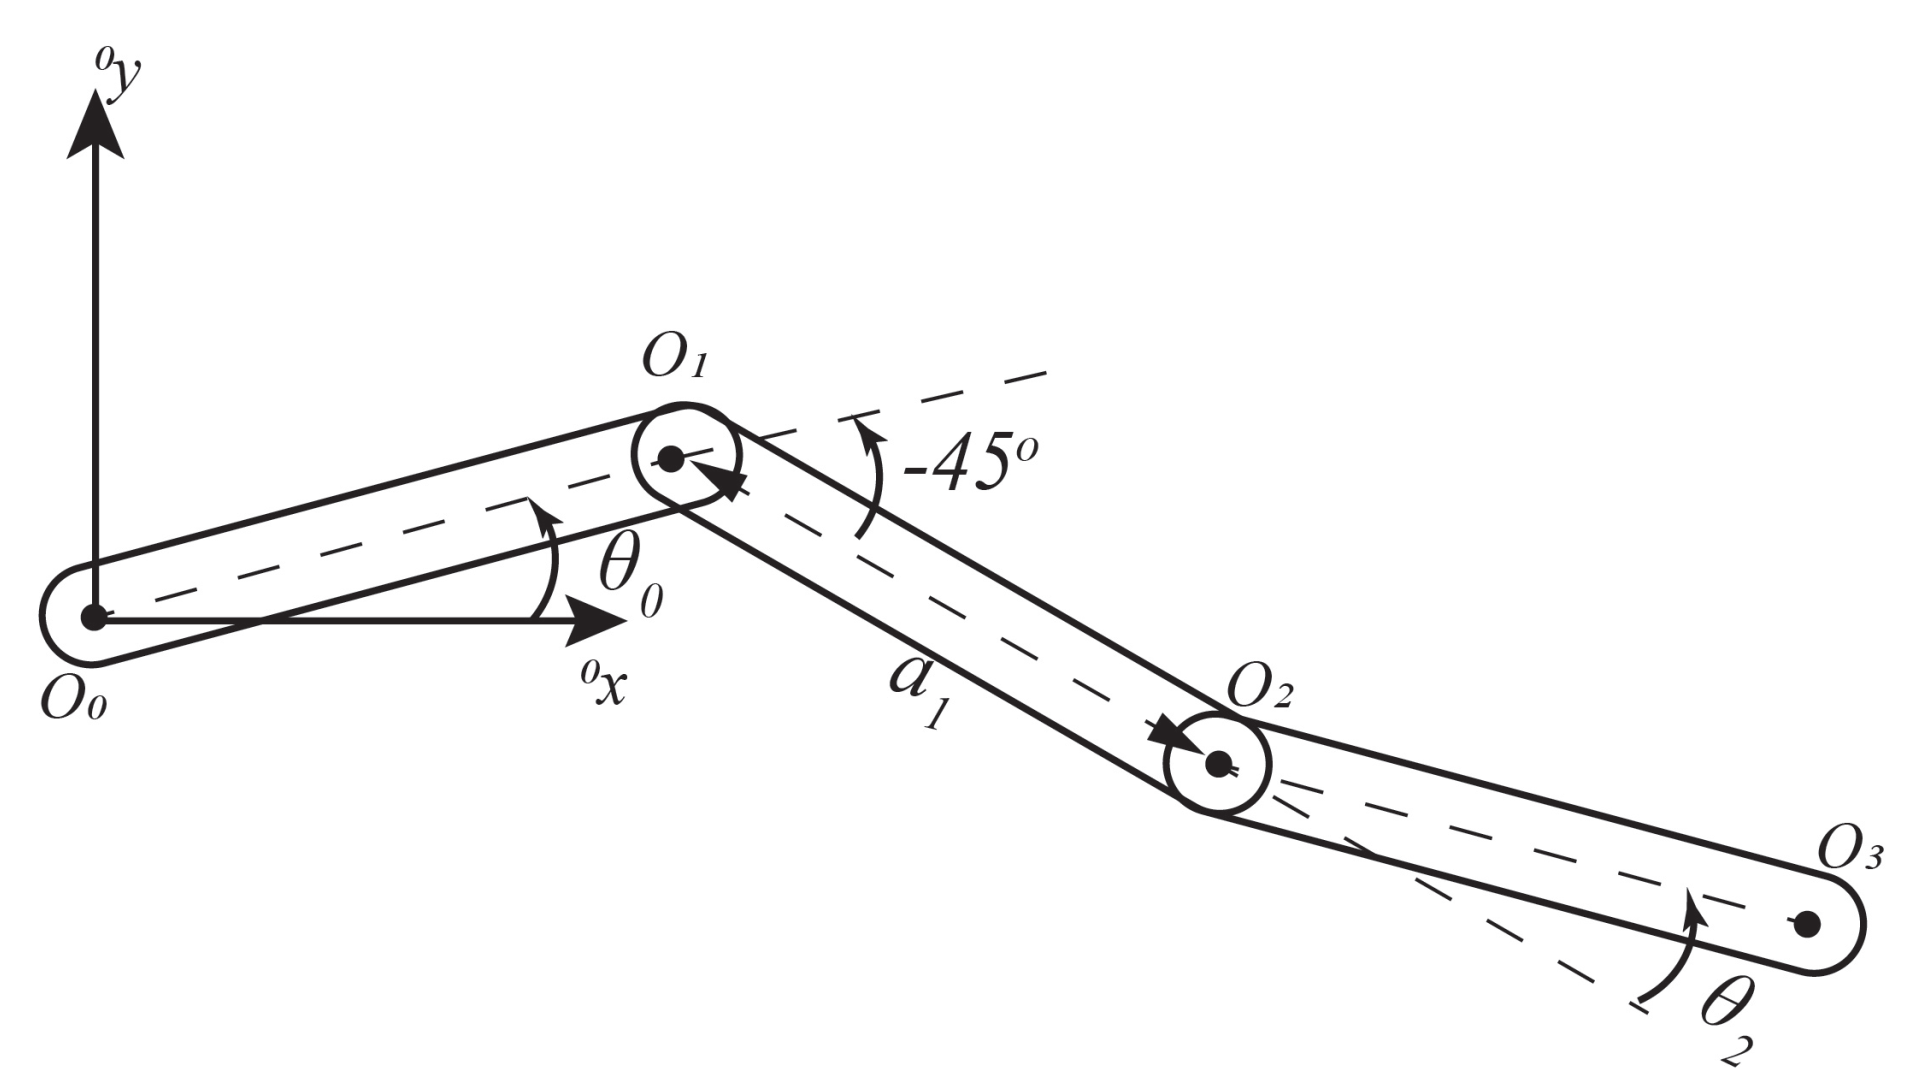
\includegraphics[width=.75\columnwidth]{figures/RPR_manipulator.png}
	\centering
	\caption{Three link RPR manipulator.}
	\label{fig:rpr}
\end{figure}

\begin{enumerate}[label=(\alph*)]
    \item Draw the manipulator when $\theta_0 = \pi/4\,$\unit{rad}; $a_1 = 0.5\,$\unit{m}; $\theta_2 = \pi/4\,$\unit{rad}, make sure you draw in and label the intermediate coordinate system directions.
    \item Let $\theta_0$ be the first joint’s angle. What is the symbolic homogeneous transformation from the world frame to the distal (far) end of link $1$, i.e., $\prescript{0}{}{\boldsymbol{T}}_{1}$?
    \item Let $a_1$ be the second joint’s length. What is the symbolic homogeneous transformation from the distal end of link $1$ to the distal end of link $2$, i.e., $\prescript{1}{}{\boldsymbol{T}}_{2}$?
    \item  Let $\theta_2$ be the third joint’s angle. What is the symbolic homogeneous transformation from the distal end of link $2$ to the distal end of link $3$, i.e., $\prescript{2}{}{\boldsymbol{T}}_{3}$?
    \item What is the symbolic homogeneous transformation from the world origin
    to the distal end of link $3$, i.e., $\prescript{0}{}{\boldsymbol{T}}_{3}$?
\end{enumerate}

 
\end{problem}

\begin{problem}{3}%theorem, exercise, problem, or question 
Figure~\ref{fig:path} shows the path of a mobile robot. The displacements are
given by: $\prescript{0}{}{\boldsymbol{d}}_{01}= \begin{bmatrix}
    2 \\ 1
\end{bmatrix}$, $\prescript{1}{}{\boldsymbol{d}}_{12}= \begin{bmatrix}
    0 \\ 0
\end{bmatrix}$, $\prescript{2}{}{\boldsymbol{d}}_{23}= \begin{bmatrix}
    2 \\ 0
\end{bmatrix}$, $\prescript{3}{}{\boldsymbol{d}}_{34}= \begin{bmatrix}
    0 \\ 0
\end{bmatrix}$, $\prescript{4}{}{\boldsymbol{d}}_{45}= \begin{bmatrix}
    0 \\ 3
\end{bmatrix}$.

\begin{figure}[!h]
	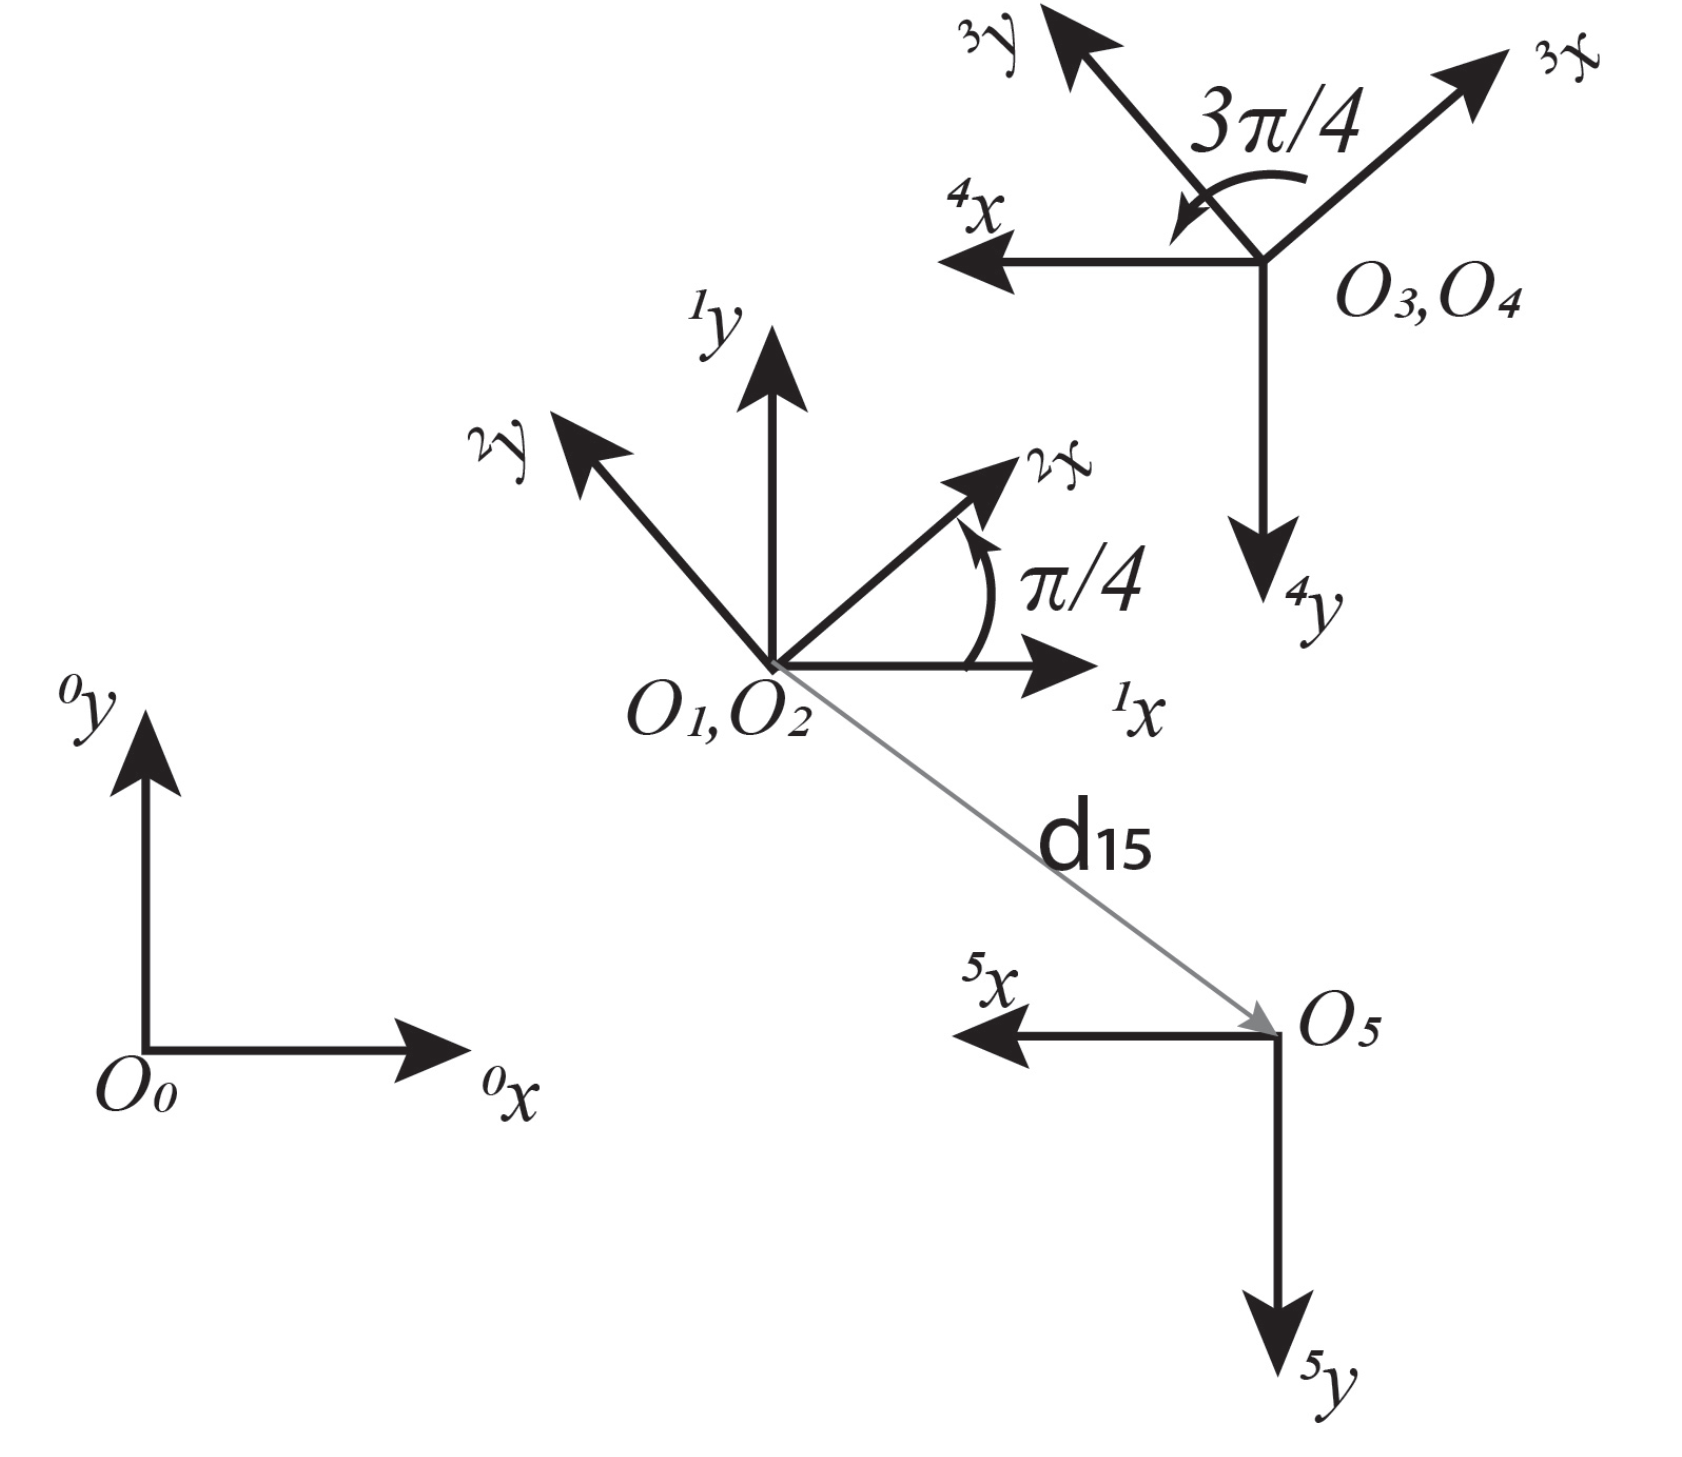
\includegraphics[width=.6\columnwidth]{figures/path_mobile_robot.png}
	\centering
	\caption{Path of mobile robot.}
	\label{fig:path}
\end{figure}

\begin{enumerate}[label=(\alph*)]
    \item Calculate: $\prescript{0}{}{\boldsymbol{T}}_{1}$
    \item Calculate: $\prescript{1}{}{\boldsymbol{T}}_{2}$
    \item Calculate: $\prescript{2}{}{\boldsymbol{T}}_{3}$
    \item Calculate: $\prescript{3}{}{\boldsymbol{T}}_{4}$
    \item Calculate: $\prescript{4}{}{\boldsymbol{T}}_{5}$
    \item Calculate: $\prescript{0}{}{\boldsymbol{T}}_{5}$
    \item Calculate: $\prescript{0}{}{\boldsymbol{d}}_{05}$
    \item Calculate: $\prescript{0}{}{\boldsymbol{R}}_{5}$ 
    \item Using homogeneous transformations,
        \begin{enumerate}[label=(\Roman*)]
            \item What is the equation in terms of homogeneous transformations to find the displacement vector from origin $1$ to origin $5$ (${\boldsymbol{d}}_{15}$) expressed in the final (Origin $5$) frame?
            \item What is this numerical displacement?
        \end{enumerate}
\end{enumerate}
 
\end{problem}

\begin{problem}{4}%theorem, exercise, problem, or question 
Determine if the following matrices are rotations and explain why or why not:
\begin{enumerate}[label=(\alph*)]
    \item $\begin{bmatrix}
        0 & 1 & 0 \\
        1 & 0 & 0 \\
        0 & 0 & 1
        \end{bmatrix} $
    \item $\begin{bmatrix}
        0 & 1 & 0 \\
        1 & 0 & 0 \\
        0 & 0 & -1
        \end{bmatrix} $
    \item $\begin{bmatrix}
        -0.254 & 0.087 & -0.963 \\
        0.967 & 0.0169 & -0.253 \\
        -0.00572 & -0.996 & -0.0884
        \end{bmatrix} $
    \item $\begin{bmatrix}
        0.546 & 0.0719 & -1.47 \\
        0.814 & -0.696 & -0.0502 \\
        -1.23 & -0.813 & 0.474
        \end{bmatrix} $
\end{enumerate}

\end{problem}
\newpage
\begin{problem}{5}%theorem, exercise, problem, or question 
Complete the below rotation matrices. How do you know it is correct?
\begin{enumerate}[label=(\alph*)]
    \item $\begin{bmatrix}
        0 & 0 & ? \\
        0 & 1 & ? \\
        1 & 0 & ?
        \end{bmatrix} $
    \item $\begin{bmatrix}
        -1 & ? & ? \\
        ? & 1 & ? \\
        ? & ? & ?
        \end{bmatrix} $
    \item $\begin{bmatrix}
        0.3698 & ? & 0.8665 \\
        -0.9276 & ? & 0.324 \\
        -0.05236 & ? & 0.3797
        \end{bmatrix} $
    \item $\begin{bmatrix}
        ? & 0.1166 & ? \\
        -0.2039 & ? & 0.2153 \\
        ? & ? & -0.3672
        \end{bmatrix} $
\end{enumerate}

\end{problem}




\end{document}